\documentclass[3pt,landscape]{article}
%ss[10pt,landscape]{article}
\usepackage{multicol}
\usepackage{calc}
\usepackage{ifthen}
\usepackage[landscape]{geometry}
\usepackage{amsmath,amsthm,amsfonts,amssymb}
\usepackage{color,graphicx,overpic}
\usepackage{hyperref}


\pdfinfo{
/Title (example.pdf)
/Creator (TeX)
/Producer (pdfTeX 1.40.0)
/Author (Seamus)
/Subject (Example)
/Keywords (pdflatex, latex,pdftex,tex)}

% This sets page margins to .5 inch if using letter paper, and to 1cm
% if using A4 paper. (This probably isn't strictly necessary.)
% If using another size paper, use default 1cm margins.
\ifthenelse{\lengthtest { \paperwidth = 11in}}
    { \geometry{top=.3in,left=.3in,right=.3in,bottom=.3in} }
    {\ifthenelse{ \lengthtest{ \paperwidth = 297mm}}
        {\geometry{top=1cm,left=1cm,right=1cm,bottom=1cm} }
        {\geometry{top=1cm,left=1cm,right=1cm,bottom=1cm} }
    }

% Turn off header and footer
\pagestyle{empty}

% Redefine section commands to use less space
\makeatletter
\renewcommand{\section}{\@startsection{section}{1}{0mm}%
                            {-1ex plus -.5ex minus -.2ex}%
                            {0.5ex plus .2ex}%x
                            {\normalfont\large\bfseries}}
\renewcommand{\subsection}{\@startsection{subsection}{2}{0mm}%
                            {-1explus -.5ex minus -.2ex}%
                            {0.5ex plus .2ex}%
                            {\normalfont\normalsize\bfseries}}
\renewcommand{\subsubsection}{\@startsection{subsubsection}{3}{0mm}%
                            {-1ex plus -.5ex minus -.2ex}%
                            {1ex plus .2ex}%
                            {\normalfont\small\bfseries}}
\makeatother

% Define BibTeX command
\def\BibTeX{{\rm B\kern-.05em{\sc i\kern-.025em b}\kern-.08em
    T\kern-.1667em\lower.7ex\hbox{E}\kern-.125emX}}

% Don't print section numbers
\setcounter{secnumdepth}{0}


\setlength{\parindent}{0pt}
\setlength{\parskip}{0pt plus 0.5ex}

%My Environments
\newtheorem{example}[section]{Example}
% -----------------------------------------------------------------------

\def\ci{\perp\!\!\!\perp}

\begin{document}
\raggedright
\footnotesize
\begin{multicols}{3}


% multicol parameters
% These lengths are set only within the two main columns
%\setlength{\columnseprule}{0.25pt}
\setlength{\premulticols}{1pt}
\setlength{\postmulticols}{1pt}
\setlength{\multicolsep}{1pt}
\setlength{\columnsep}{2pt}

\begin{center}
    \Large{\underline{CS 161 Final Cheat Sheet}} \\
\end{center}

\subsubsection*{Kerchoff's Principle}
You should not rely on the secrecy of the algorithm/protocol and or keysize, as wall as the possible plain text for security because eventually the adversary will figure them out.

\subsubsection*{Mono-Alphabetic Ciphers: 1 to 1 mapping of characters to symbols}
\begin{itemize}
    \item Subsitution
        \begin{itemize}
            \item Shift or Caesar's Cipher
                \(E_{k}(m) \leftarrow m+k(\texttt{mod } N)\)
                \(D_{k}(c) \leftarrow c-k(\texttt{mod } N)\)
            \item Affine Cipher:
                \(E_{k}(m) \leftarrow k_{!}m+k_{2}(\texttt{mod } N)\)
                \(D_{k}(c) \leftarrow k_{!}^{-1}(c-k(\texttt{mod } N)\)
            \item Substitution Ciphers have an extreme vulnerability to frequency attacks.
        \end{itemize}
\end{itemize}

\subsubsection*{Poly-Alphabetic Ciphers}
\begin{itemize}
    \item Vigenere Cipher: Shift by a repeated key
    \item Book Cipher (Beale Cipher) key is hidded in a passage of a set book.
    \item Vernam Cipher
        \begin{itemize}
            \item Message is m bits and the key is n bits.
            \item Bitwise xor the message and the key, if m is greater than n, then use the key multiple times.
        \end{itemize}
    \item One-Time Pad
        \begin{itemize}
            \item Same idea as the Vernam Cipher except we use a key that is the same length or greater than the length of the message, then discard it after each use.
        \end{itemize}
    \item Transposition/Permutation Cipher
        \begin{itemize}
            \item Break the message into n bit blocks, then on each block perfom the same permutation
            \item Despite being polyalphabit, the cipher is still vulnerable to frequency attacks. Because the original patterns are still basically present. You can attack by checking anagrams.
        \end{itemize}
\end{itemize}

\subsection*{Data Encryption Standard (DES)}
DES is a block cipher in which messages are divided into data blocks of a fixed length and each block is treated as one message either in M or in C. The DES encryping and decryption algorithms take as an input a 64-bit plaintext or ciphertext message and a 56-bit key, and output a 64-bit ciphertext or plaintext message.
DES is done in 3 steps:
\begin{enumerate}
    \item Apply a fixed "initial permutation" IP to the input block.
        \((L_0,R_0) \leftarrow IP(\texttt{Input Block})\) 
        This step has no apparent cryptographic significance.
    \item Iterate the following 16 rounds of operations (Feistel Cipher)\\
        \begin{center}
        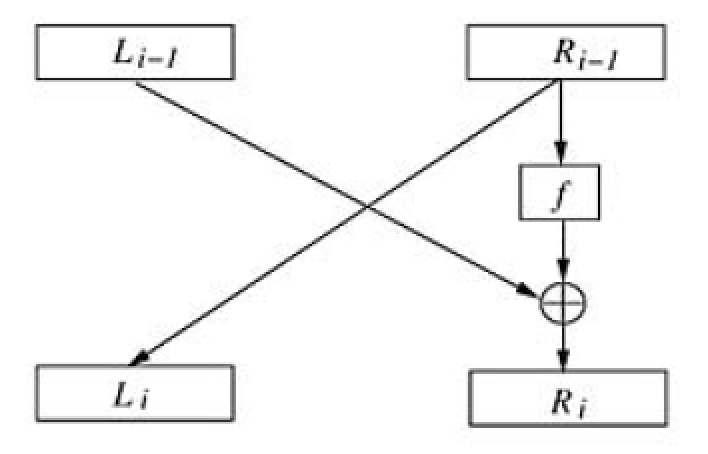
\includegraphics[scale=.47]{feistel}
        \end{center}
        \begin{itemize}
            \item the function is nonlinear and is considered a Substitution Cipher
            \item the move from \(L_{i} \rightarrow R_{i-1}\) is a Transposition cipher
            \item Vernam cipher is used at the xor
            \item k is a 48 bit subsection of the 56 bit, "round key"
        \end{itemize}
\end{enumerate}

\subsubsection*{Single DES}
\begin{itemize}
    \item vulnerable to brute force or exaustive key search attacks
\end{itemize}

\subsubsection*{Triple DES}
Triple DES uses an encryption-decryption-encryption scheme,\\
\(c \leftarrow E_{k_{1}}(D_{k_{2}}(E_{k_{1}}(m)))\)\\
\(m \leftarrow D_{k_{1}}(E_{k_{2}}(D_{k_{1}}(m)))\)\\
This scheme enlarges the keyspace while maintaining backward compatibility with single DES if \(k_{1}=k_{2}\)\\

\subsection*{Advanced Encryption Standard (AES)}
AES is a block cipher with variable block size and variable keysize. (block size can be 128, 192, 256 bit)\\
AES has 4 states:
\begin{enumerate}
    \item Sub Bytes State: nonlinear substitution on each byte
    \item Shift Rows State: Transposition rearranges the order of elements in each row
    \item Mix Columns State: Polynomial multiplication after converting column to polynomial.
    \item Add Round Key State: adds elements of round key to the state, basically bitwise "OR"
\end{enumerate}
Decryption is the inverse of these steps.

\subsubsection*{Confidentiality Modes of Operation}
Different modes of operation have been devised on top of an underlying block cipher algorithm
\begin{itemize}
    \item Electronic Codebook (ECB) Mode
        This mode encrypts and decrypts every block seperately. It is deterministic and leaves patterns in the cipher text. (for example images.)
    \item Cipher Block Chaining (CBC) Mode
        \begin{itemize}
            \item This is the most common mode of operation. In this mode the output is a sequence of n-bit cipher blocks which are chained together so that each cipher block is dependent on all the previous data blocks.
            \item Decryption can be done in parallel
            \item CBC cannot prived data integrity protection.
            \item If the CBC claims data integrity protection, Eve can use (Bomb Oracle Attack) a Decryption Oracle to figure out the padding scheme and eventually the last byte of the cipher text.
        \end{itemize}
\end{itemize}
\begin{center}
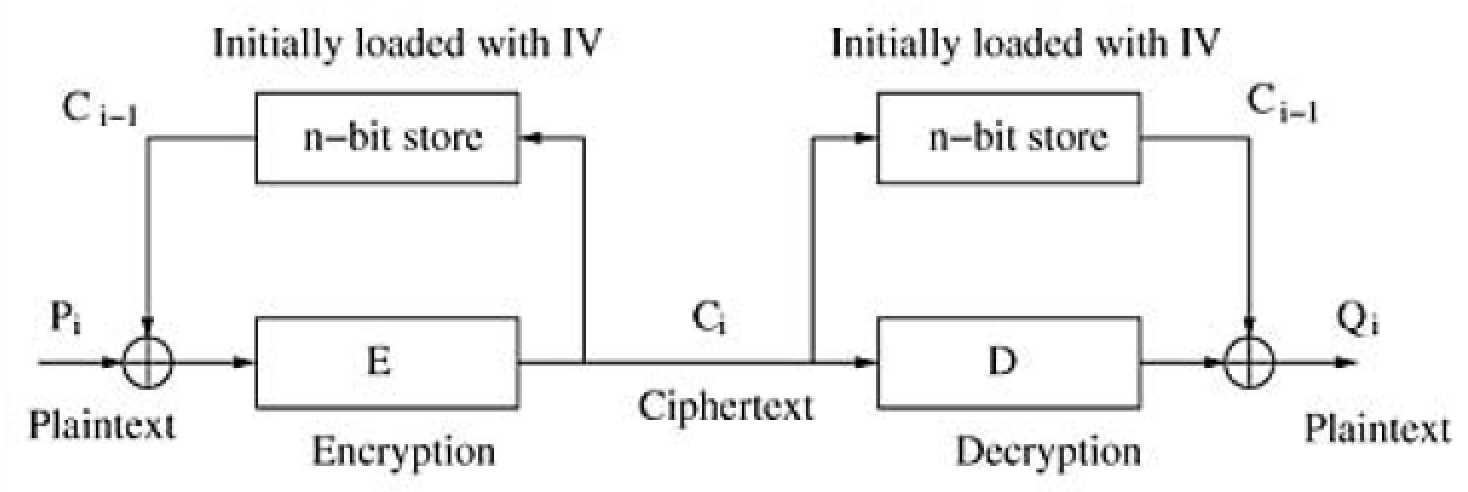
\includegraphics[scale=.33]{CBCMode}
\end{center}
\begin{itemize}
    \item Cipher Feedback (CFB) Mode
        \begin{itemize}
            \item CFB mode of opration features feeding successive cipher segments which are output from the mode back as input to the underlying block cipher algorithm.
            \item CFB requires an IV as the initial n-bit input block
        \end{itemize}
\end{itemize}
\begin{center}
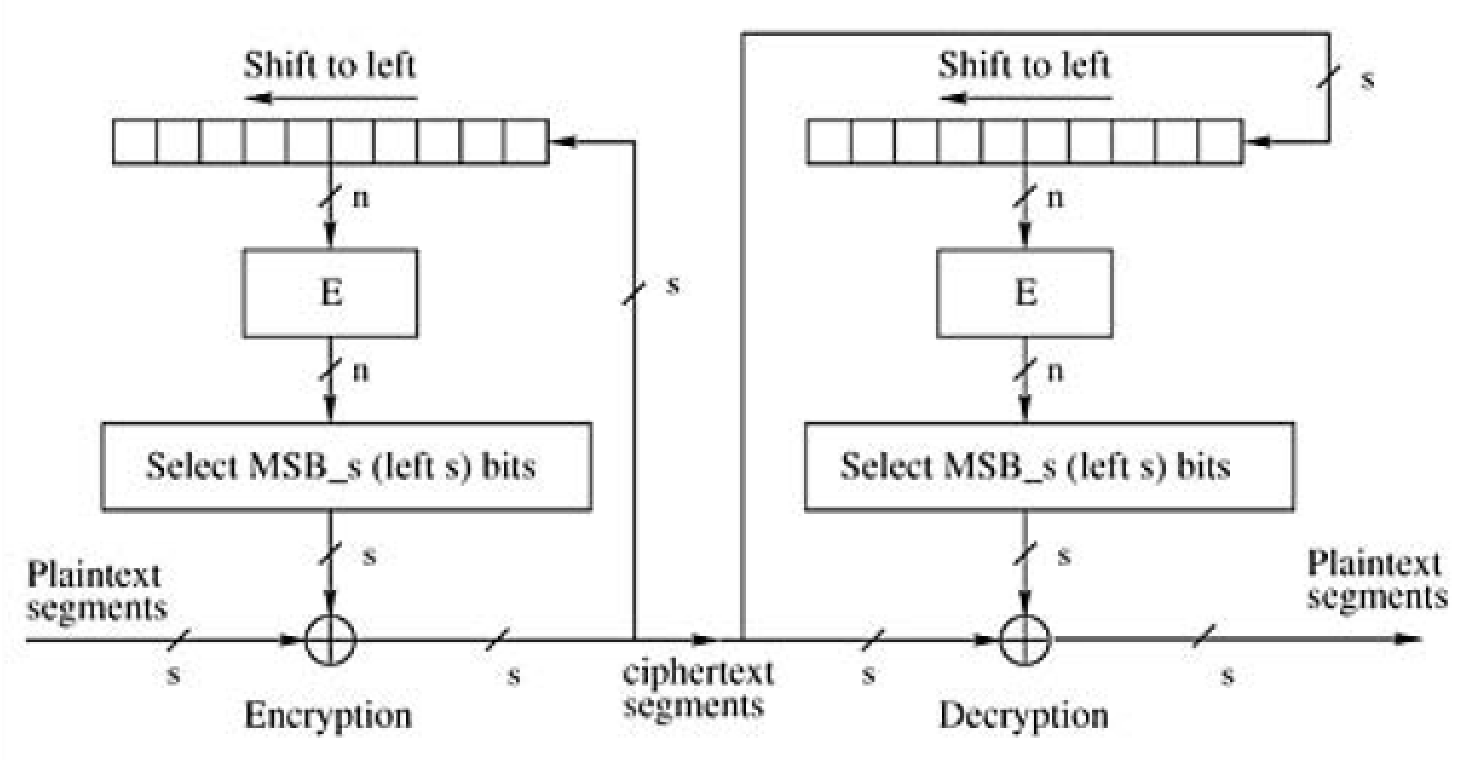
\includegraphics[scale=.35]{CFBMode}
\end{center}
\begin{itemize}
    \item Output Feedback (OFB) Mode
        \begin{itemize}
            \item The OFB mode feeds successive output blocks from the underlying block cipher back to it.
            \item The feedback blocks form a string of bits which used as the key stream of the Vernam cipher.
        \end{itemize}
\end{itemize}
\begin{center}
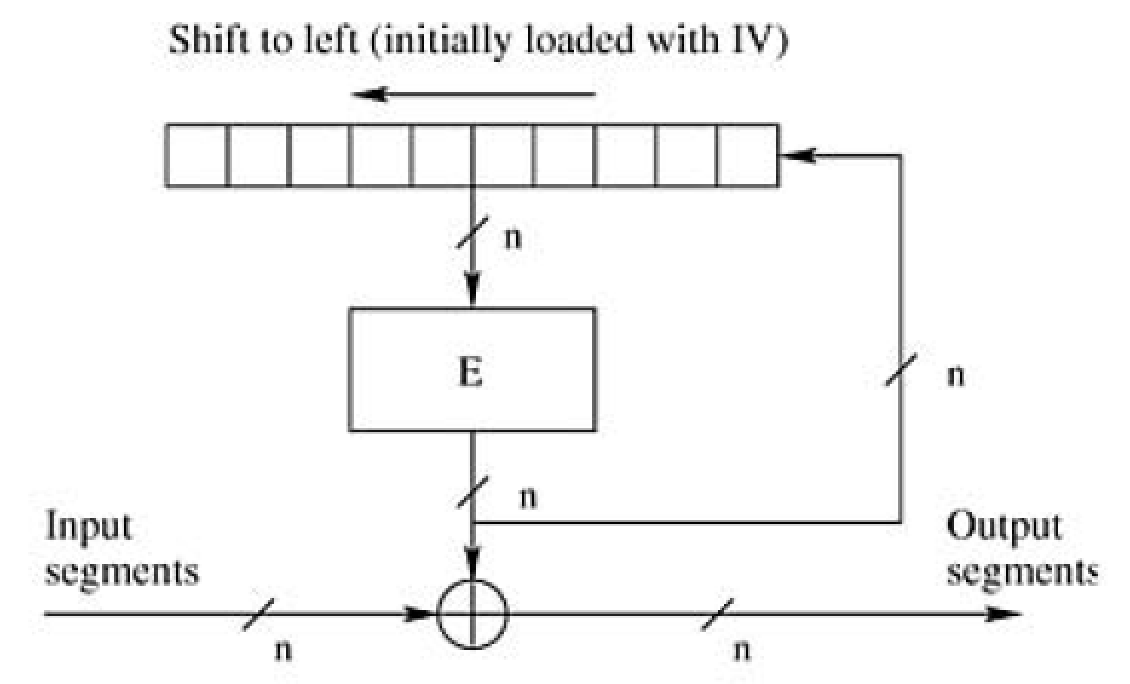
\includegraphics[scale=.32]{OFBMode}
\end{center}
\newpage
\begin{itemize}
    \item Counter (CTR) Mode
        \begin{itemize}
            \item The CTR mode features feeding the underlying block cipher algorithm with a counter value which counts up from an initial value. With a counter counting up, the underlying block cipher algorithm outputs successive blocks to form a string of bits. This string of bits is used as the key stream of the vernam cipher, that is, the key stream is XOR-ed with the plaintext blocks.
                \(C_{i} \leftarrow P_{i} \oplus E(Ctr_{i}, i=1,2,\ldots,m\)\\
                \(P_{i} \leftarrow C_{i} \oplus E(Ctr_{i}, i=1,2,\ldots,m\)
        \end{itemize}
\end{itemize}

\subsubsection*{Bomb Oracle Attack}
% todo

\subsection*{Asymmetric Cryptography}
\subsubsection*{Oneway Trapdoor Function}
\begin{itemize}
    \item Asymmetric crypto system, Public Key Cryptography
    \item \(D \rightarrow R\) is oneway, it is easy to evaluate \(\forall x \in D\) and difficult to invert for all values in R.
\end{itemize}

\subsubsection*{Textbook Encryption Algorithms}
\begin{itemize}
    \item All or Nothing Secrecy: Given Cipher Text the attacker must not be able to get any information about the plain text
    \item Passive Attacker: The attacker doesn't modify or manipulate ciphertexts they also don't ask for encryption or Decryption services. % todo check definition and move to it's own section
\end{itemize}

\subsubsection*{Diffie-Hellman Key Exchange Protocol}
\(\begin{array}{ll}
    \texttt{Common Input} & (p,g):p \texttt{ is a large prime, g is a generator}\\
    \texttt{ } & \texttt{element in } F_{p}^{*}\\
    \texttt{Output} & \texttt{An element in } F_{p}^{*} \texttt{ shared between Alice}\\
    \texttt{ } & \texttt{Bob.}
\end{array}\)
\begin{enumerate}
    \item Alice picks \(a \in U(1,p-1)\); computes \(g_{a} \leftarrow g^{a}(\texttt{mod } p)\); sends \(g_{a}\) to Bob.
    \item Bob picks \(b \in U(1,p-1)\); computes \(g_{b} \leftarrow g^{b}(\texttt{mod } p)\); sends \(g_{b}\) to Alice.
    \item Alice computes \(k \leftarrow g_{b}^{a}(\texttt{mod } p)\)
    \item Bob computes \(k \leftarrow g_{a}^{b}(\texttt{mod } p)\)
\end{enumerate}
Alice and Bob both compute the same key,
\[k = g^{ba}(\texttt{mod }p) = g^{ab}(\texttt{mod }p)\]
P is a public 2048 bit prime number.

\subsubsection*{Man in the Middle Attack on Diffie-Helman}
\begin{center}
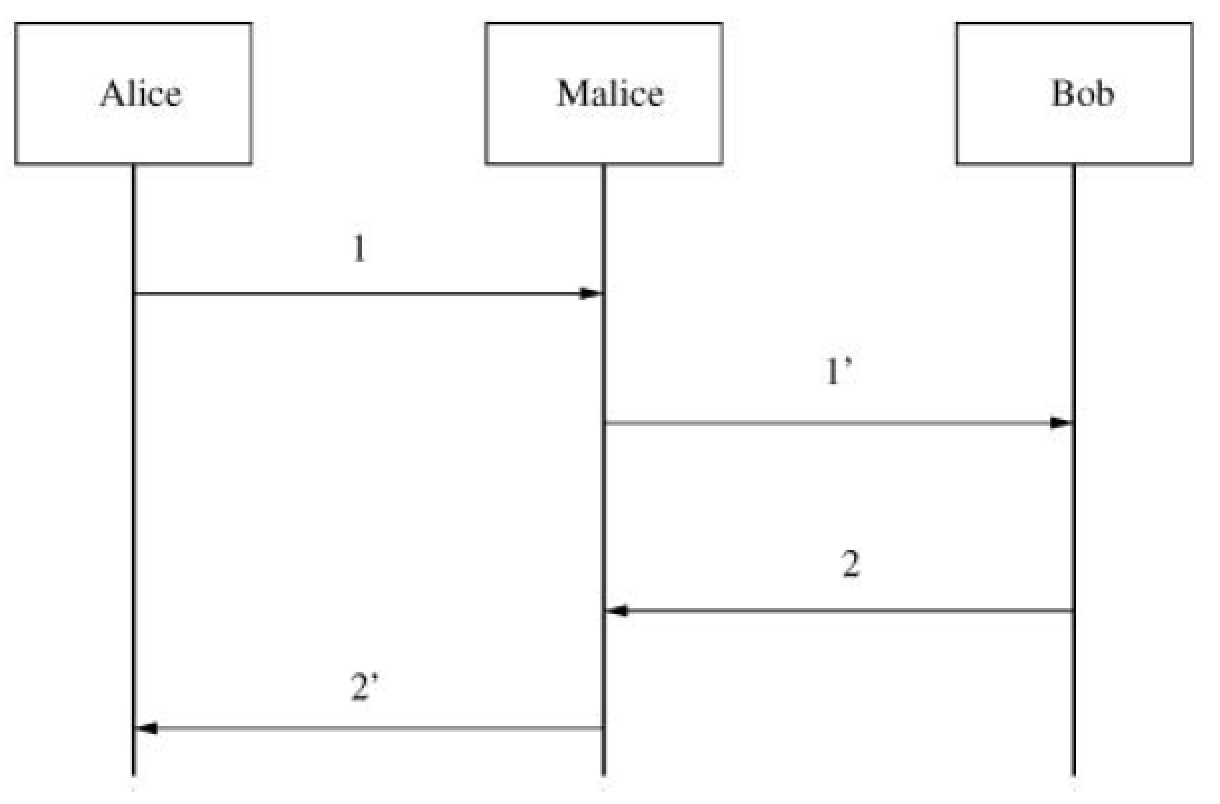
\includegraphics[scale=.26]{DiffieHelmanMITM}
\end{center}
\begin{enumerate}
    \item Alice picks a \(\in _{u}[1,p-1)\), computes \(g_{a} \leftarrow g^{a}(\texttt{mod }p)\) she sends \(g_{a}\) to Malice("bob");
    \item (1') Malice("Alice") computes \(g_{m} \leftarrow g^{m}(\texttt{mod })\) for some \(m \in [1,p-1)\); he sends \(g_{m}\) to Bob;
    \item (2) Bob picks \(b \in _{U}[1,p-1)\), computes \(g_{b} \leftarrow g^{b}(\texttt{mod }p)\); he sends \(g_{b}\) Malice("Alice");
        \item (2') Malice("Bob") sends to Alice: \(g_{m}\);
        \item (3) Alice computes \(k_{1} \leftarrow g^{a}_{m}(\texttt{mod }p)\);
        \item (4) Bob computes \(k_{2} \leftarrow g^{b}_{m}(\texttt{mod }p)\);
\end{enumerate}

\subsubsection*{Diffie-Helman and the Discrete Logarithm Problem}
\begin{itemize}
    \item Computational Diffie-Hellman Problem
        % \(\begin{array}{ll}
        %     \texttt{INPUT} & \texttt{desc}(F_{q}): \texttt{the description of finite field } F_{q}
        %     \texttt{ } & g \in F^{*}_{q:a}
        % \end{arry}\)
    \item Discrete Logarithm Problem
        % \texttt{OUTPUT} & \texttt{the unique integer } (a<q) \texttt{ such that } h = g^{a}
\end{itemize}

% You can even have references
\rule{0.3\linewidth}{0.25pt}
\scriptsize
\bibliographystyle{abstract}
\bibliography{refFile}
\end{multicols}
\end{document}
